[programmer/prog-gui.tex]
\section{GUI Guide lines}
The \dabc\ GUI is written in Java. In the following we refer to it
as a whole as \gui. 
It uses the DIM Java package to register the
DIM services provided by the \dabc\ DIM servers. 
It is generic in that it
builds most of the panels from the services available.
Thus it can control and monitor any system running DIM servers conforming to
rules described in the following. 
According the description above it does the following:
\begin{compactitem}[$\bullet$]
\item Get list of commands and parameters and create objects for each.
\item Put parameters in a table.
\item Put commands in a command tree.
\item Create graphics panels for rate meters, states, histograms, and infos.
\end{compactitem}

\section{DIM Usage}
\index{DIM!Introduction}
DIM is a light weight communication protocoll based on publish/subscribe mechanism. Servers publish named services (commands or parameters) to a DIM name server. Clients can subscribe such services by name. They then get the values of the services subscribed from the server providing it. Whenever a server updates a service, all subscribed clients get the new value. Clients can also execute commands on the server side.

DIM provides the possibility to specify parameters and command arguments as primitives (I or L,X,C,F,D) or structures. The structures are described in a format string which can be retrieved by the clients (for parameters and commands) and servers (for commands):
\begin{verbatim}
   T:s;T:s;T:s ...
\end{verbatim}
Thus a client can generically access parameter structures, but without semantical interpretation.
In addition to the data and format string one longword called \verba{quality} is sent.

\subsection{\dabc\ DIM naming conventions}
\index{DIM!Conventions}
\index{DABC!DIM conventions}
When the number and kind of services of DIM servers often change it would be very convenient if a generic GUI would show all available services without further programming. It would be also very nice if standard graphical elements would be used to display certain parameters like rate meters. If we have many services it would be convenient to have a naming convention which allows to build tree structures on the GUI.

Naming conventions for generic \gui\ (line breaks for better reading):
{\small \begin{verbatim}
   /servernamespace
   /nodename[:nodeID]
   /[[applicationnamespace::]applicationname:]applicationID
   /[TYPE.module.]name
Example:
   /DABC/lx05/Control/RunState
\end{verbatim}
}
We recommend to forbid spaces in any name fields. Dots should not be used except in names (last field). The generic \gui\ can handle only services from one server name space 
(defined by \keyw{DIM\_DNS\_NODE}). For \dabc\ and \mbs\ this servernamespace is set to \keyw{DABC}.
\subsection{\dabc\ DIM records}
For generic GUIs we need something similar to the EPICS records. This means to define structures which can be identified. How shall they be indentified? One possibility would be to prefix a type to the parameter name, i.e. \verba{rate:DataRate}. Another to use the quality longword. This longword can be set by the server. One could mask the bytes of this longword for different information:
{\small \begin{verbatim}
   mode (MSB)| visibility | type | status (LSB)
   mode: not used
   visibility: Bit wise (can be ORed)
     HIDDEN    = all zero
     VISIBLE   = 1  appears in parameter table
     MONITOR   = 2  in table, graphics shown automatically 
                    if type is STATE, RATE or HISTOGRAM
     CHANGABLE = 4  in table, can be modified
     IMPORTANT = 8  in table also if GUI has a "minimal" view.
   type: (exclusive)
     PLAIN     = 0
     GENERIC   = 1
     STATE     = 2
     RATE      = 3
     HISTOGRAM = 4
     MODULE    = 5
     PORT      = 6
     DEVICE    = 7
     QUEUE     = 8
     COMMANDDESC= 9
     INFO      = 10
   status: (exclusive) 
     NOTSPEC     = 0
     SUCCESS     = 1
     INFORMATION = 2
     WARNING     = 3
     ERROR       = 4
     FATAL       = 5
\end{verbatim}
}

Then we could provide at the client side objects for handling and visualization of such records.

\subsubsection{Record ID=0: Plain}

Scalar data item of atomic type

\subsubsection{Record ID=1: Generic self describing}
For these one would need one structure per number of arguments. Therefore the generic type would be rather realized by a more flexible text format, like XML. This means the DIM service has a string as argument which must be parsed to get the values.
\begin{compactdesc}
\item[XML schema] char, similar to command descriptor.
\item[Format:] C
\end{compactdesc}

\subsubsection{Record ID=2: State}
\begin{compactdesc}
\item[severity] int, 0=Success, 1=warning, 2=error, 3=fatal)
\item[color] char, (Red, Green, Blue, Cyan, Magenta, Yellow)
\item[state] char, name of state
\item[Format:] L:1;C:16;C:16
\end{compactdesc}

\subsubsection{Record ID=3: Rate}
\begin{compactdesc}
\item[value]   float 
\item[displaymode ]   int, (arc, bar, statistics, trend)
\item[lower limit]   float 
\item[upper limit]   float 
\item[lower alarm]   float
\item[upper alarm]   float 
\item[color]   char,  (Red, Green, Blue, Cyan, Magenta, Yellow)
\item[alarm color]   char,  (Red, Green, Blue, Cyan, Magenta, Yellow)
\item[units]   char 
\item[Format:] F:1;L:1;F:1;F:1;F:1;F:1;C:16;C:16;C
\end{compactdesc}

\subsubsection{Record ID=4: Histogram}
Structure must be allocated including the data field witch may be integer or double.
\begin{compactdesc}
\item[channels]   int 
\item[lower limit]   float 
\item[upper limit]   float 
\item[axis lettering]   char 
\item[content lettering]   char 
\item[color]   char, (White, Red, Green, Blue, Cyan, Magenta, Yellow)
\item[first data channel]   int 
\item[Format:] L:1;F:1;F:1;C:32;C:32;C:16;I(or D)
\end{compactdesc}

\subsubsection{Record ID=10: Info}
\begin{compactdesc}
\item[verbose]   int,  (0=Plain text, 1=Node:text)
\item[color]   char,  (Red, Green, Blue, Cyan, Magenta, Yellow)
\item[text]   char,  line of text
\item[Format:] L:1;C:16;C:128
\end{compactdesc}

\subsubsection{Record ID=9: Command descriptor}
This is an invisible parameter describing a command argument list. The service name must be correlated with the command name, e.g. by trailing underscore.
\begin{compactdesc}
\item[description]   char,  XMl string describing arguments
\item[Format:] C
\end{compactdesc}

The descriptor string could be XML specifying the argument name, type, required and description. Question if default value should be given here for optional arguments. Example:
{\small \begin{verbatim}
<?xml version="1.0" encoding="utf-8"?>
<command name="com1" scope="public" content="default">
<argument name="arg1" type="F" value="1.0" required="req"/>
<argument name="arg2" type="I" value="2" required="opt"/>
<argument name="arg3" type="C" value="def3" required="req"/>
<argument name="arg4" type="boolean" value="" required="opt"/>
</command>
\end{verbatim}
}
The command definition can be used by the \gui\ to build input panels for commands. The \verba{scope} can be used to classify commands, \verba{content} should be set to \keyw{default} if argument values are default, \keyw{values} if argument values have been changed.
\subsubsection{Commands}
Commands have one string argument only. This leaves the arguments to semantic definitions in string format. To implement a minimal security, the first 14 characters of the argument string should be an encrypted password (13 characters by crypt plus space). The arguments are passed as string. A command structure could look like:
\bdes
\item[password]   char[14]
\item[argument]   char,  string
\item[Format:] C
\edes
The argument string has the same XML as the command description. Thus, the same parser can be used to encode/decode the description (parameter) and the command. An alternate format is the \mbs\ style format \verba{argument=value} where boolean arguments are given by \verba{-argument} if argument is true.
\subsubsection{Setting parameters}
If a parameter should be changable from the \gui, there must be a command for that. A fixed command \comm{SetParameter} must be defined on the server for that. 
Argument is a string of form \verba{name=value}. In the parameter table of the \gui\ one field can be provided to enter a new value and the command \comm{SetParameter} is used to set the new value.
\subsection{Application servers}
Any application which can implement DIM services can be controlled by the generic \gui\ if it follows the protocol described above. The first application was \dabc, the second one \mbs.
\subsection{\dabc\ GUI usage of DIM}
The service names follow a structured syntax as described above. The name fields are used to
build trees (for commands). Using the DIM quality longword (delivered by the server together
with each update) simple aggregated data services (records) are defined.
Currently the records \\
\keyw{STATE}, \keyw{RATE}, \keyw{HISTOGRAM}, \keyw{COMMANDDESC} and \keyw{INFO}.\\
are used. When the \gui\ receives the first update of a service (immediately after subscribing)
it can determine the record type and handle the record in an appropriate way.
The \keyw{COMMANDDESC} record is an XML string describing a command.
The name of a descriptor record must be the name of the command it describes followed by an underscore.
\section{GUI global layout}
The top window of the \gui\ is a \class{JFrame}. Inside that is a \class{JPanel}
which contains on top a \class{JToolBar} (all the main buttons), 
in the middle a \class{JDesktopPane} (main viewing area), and at the bottom
a \class{JTextArea} (One line text for server list). 
All other windows are inside (added to) the desktop as \class{JInternalFrame}s.
Typically such a frame contains again a \class{JPanel}. Inside that panel various
different layouts can be used like \class{JSplitPane}, or a \class{Jtree} in a \class{JScrollPane}.
In fact, \class{xInternalFrame}, a subclass of \class{JInternalFrame} is used.
It can contain exactly one panel, has a mechanism to store and restore its size and position,
and implenents the callback functions for resizing and closing.

Inside the internal frames two types of panels are often used: prompter panels and
graphics panels.
\subsection{Prompter panels}
Prompter panels can be implemented subclassing class \class{xPanelPrompt}.
The layout is in rows. A row can be a prompter line (\class{JLabel} label and \class{JTextField} input field),
a text button \class{JButton}, or a \class{JLabel} label and \class{JCheckBox}. At the bottom there is a \class{JToolBar}
where buttons with icons can be placed. The prompter class must implement the 
\class{ActionListener}, ie. provide the \func{actionPerformed} function which is
the central call back function for all elements.
\subsection{Graphics panels}
Graphics panels are provided by class \class{xPanelGraphics}.
The layout is as a matrix with columns and rows. All items to be added 
must be \class{JPanel}s and implement \class{xiPanelItem} (see below).
The items are added line by line. The number of items per line (columns)
is a parameter. All items must have the same size.
Currently no menu bar is supported.
\section{GUI Panels}
Brief description of panels implemented in the \gui.
\subsection{\dabc\ launch panel}
\class{xPanelDabc} extending \class{xPanelPrompt}.\\
Form to enter all information needed to startup \dabc\ tasks and
buttons to execute standard commands.
The values of the form (internally stored in \class{xFormDabc} extending of \class{xForm})
can be saved to an XML file and are restored from it. File name is either
\verba{DabcLaunch.xml} or translation of \keyw{DABC\_LAUNCH\_DABC}, respectively.
\subsection{\mbs\ launch panel}
\class{xPanelMbs} extending \class{xPanelPrompt}.\\
Form to enter all information needed to startup \mbs\ tasks and
buttons to execute standard commands.
The values of the form (internally stored in \class{xFormMbs} extending of \class{xForm})
can be saved to an XML file and are restored from it. File name is either
\verba{MbsLaunch.xml} or translation of \keyw{DABC\_LAUNCH\_MBS}, respectively.
\subsection{Combined \dabc\ and \mbs\ launch panel}
\class{xPanelDabcMbs} extending \class{xPanelPrompt}.\\
It is a combination of both, \dabc\ and \mbs\ launch panel.
\subsection{Parameter table}
\class{xPanelParameter} extending \class{JPanel}.\\
Is rebuilt from scratch by \class{xDesktop} whenever the DIM service list has been updated.\\
The panel gets the list of parameters (\class{xDimParameter}) from the DIM browser (\class{xDimBrowser}). It builds a table from all visible parameters.
It creates a list of command descriptors (\class{xXmlParser}).
\subsection{Parameter selection panel}
\class{xPanelSelect} extending \class{xPanelPrompt}.\\
This form can be used to specify various filters on parameter attributes.
Parameters matching the filters are shown in a separate frame. Values
are updated on DIM update and can be modified interactively.
\subsection{Command panel}
\class{xPanelCommand} extending \class{JPanel}.\\
Is rebuilt from scratch by \class{xDesktop} whenever the DIM service list has been updated.\\
This panel is split into a right and a left part. On the left, there is the command tree,
on the right the argument prompter panel for the currently selected command.
The panel gets the list of commands (\class{xDimCommand}) from the DIM browser (\class{xDimBrowser}).
The list of command descriptors (\class{xXmlParser}) is copied in \class{xDesktop} from \class{xPanelParameter} to
\class{xPanelCommand} and the \class{xXmlParser} objects are added to the
\class{xDimCommand} objects they belong to.
\subsection{Monitoring panels}
These panels are very similar to \class{xPanelGraphics} but have additional
functionality. 
\index{TODO!xPanelGraphics}\strong{TODO:} In the future, \class{xPanelGraphics} should be extended to provide all that functionality, or at least serves as base class.
\bdes
\item [\class{xPanelMeter}:]  \class{JPanel}, for rate meters (\class{xMeter})
\item [\class{xPanelState}:]  \class{JPanel}, for states (\class{xState})
\item [\class{xPanelInfo}:]   \class{JPanel}, for infos (\class{xInfo})
\item [\class{xPanelHisto}:]  \class{JPanel}, for histograms (\class{xHisto})
\edes
The monitoring panels contain special graphics objects:
\subsubsection{\class{xMeter}}
Displays a changing value between limits as rate meter, bar, histogram or trend.
With the right mouse a context menu is popped up where one can switch between these
modes. One also can change the limits, autoscale mode (limits are adjusted dynamically),
and the color.
\subsubsection{\class{xRate}}
Displays a changing value between limits as bar. Very compact with full name.
\subsubsection{\class{xState}}
Displays a severity as colored box together with a brief text line.
\subsubsection{\class{xHisto}}
Displays a histogram.
\subsubsection{\class{xInfo}}
Displays a colored text line.
\subsection{Logging window}
\class{xPanelLogger} extending \class{JPanel}.\\
Central window to write messages.
\section{GUI save/restore setups}
There are several setups which can be stored in XML files and are retrieved
when the \gui\ is started again.
\bdes
\item [\keyw{DABC\_LAUNCH\_DABC}]: 
Values of \dabc\ launch panel. Saved by button in panel. \\
Default \verba{DabcLaunch.xml}.
\item [\keyw{DABC\_LAUNCH\_MBS}]: 
Values of \mbs\ launch panel. Saved by button in panel. \\
Default \verba{MbsLaunch.xml}.
\item [\keyw{DABC\_RECORD\_ATTRIBUTES}]: 
Attributes of records. Saved by main save button. \\
Default \verba{Records.xml}.
\item [\keyw{DABC\_PARAMETER\_FILTER}]: 
Values of parameter filter panel. Saved by main save button. \\
Default \verba{Selection.xml}.
\item [\keyw{DABC\_GUI\_LAYOUT}]: 
Layout of frames. Saved by main save button. \\
Default \verba{Layout.xml}.
\edes
\subsection{Record attributes}
File {\tt Records.xml}
{\small \begin{verbatim}
<?xml version="1.0" encoding="utf-8"?>
<Record>
<Meter name="DABC/X86-7/MSG/DataRateKb" 
       visible="true" 
       mode="0" 
       auto="false" 
       log="false" 
       low="00000000.0" 
       up="00016000.0" 
       color="Red"/>
</Record>
\end{verbatim}
}
\subsection{Parameter filter}
File {\tt Selection.xml}
{\small \begin{verbatim}
<?xml version="1.0" encoding="utf-8"?>
<Selection>
<Full contains="Date" filter="false" />
<Node contains="X86-7" filter="false" />
<Application contains="MSG" filter="false" />
<Name contains="*" filter="false" />
<Records Only="true"  Rates="true"  States="false"  Infos="false" />
</Selection>
\end{verbatim}
}
\subsection{Windows layout}
File {\tt Layout.xml}
{\small \begin{verbatim}
<?xml version="1.0" encoding="utf-8"?>
<Layout>
<WindowLayout>
<Main shape="357,53,857,953" columns="0" show="true"/>
<Command shape="0,230,650,200" columns="0" show="false"/>
<Parameter shape="20,259,578,386" columns="0" show="false"/>
<Logger shape="0,650,680,150" columns="0" show="false"/>
<Meter shape="463,13,413,236" columns="4" show="false"/>
<State shape="85,504,313,206" columns="2" show="false"/>
<Info shape="521,482,613,217" columns="1" show="false"/>
<Histogram shape="124,508,613,206" columns="3" show="false"/>
<DabcLauncher shape="0,0,100,100" columns="0" show="false"/>
<MbsLauncher shape="50,14,404,272" columns="0" show="false"/>
<DabcMbsLauncher shape="0,0,430,424" columns="0" show="false"/>
<ParameterSelect shape="300,0,271,326" columns="0" show="true"/>
<ParameterList shape="13,364,810,426" columns="1" show="true"/>
</WindowLayout>
<TableLayout>
<Parameter width="74,74,74,74,74,74,74,74" />
</TableLayout>
</Layout>
\end{verbatim}
}
\subsection{\dabc\ launch panel values}
File {\tt DabcLaunch.xml}
{\small \begin{verbatim}
<?xml version="1.0" encoding="utf-8"?>
<DabcLaunch>
<DabcMaster prompt="DABC Master" value="lx100.gsi.de" />
<DabcName prompt="DABC Name" value="Controller:41" />
<DabcUserPath prompt="DABC user path" value="myWorkDir" />
<DabcSystemPath prompt="DABC system path" value="/dabc" />
<DabcSetup prompt="DABC setup file" value="SetupDabc.xml" />
<DabcScript prompt="DABC Script" value="ps" />
<DabcServers prompt="%Number of needed DIM servers%" value="5" />
</DabcLaunch>
\end{verbatim}
}
\subsection{\mbs\ launch panel values}
File {\tt MbsLaunch.xml}
{\small \begin{verbatim}
<?xml version="1.0" encoding="utf-8"?>
<MbsLaunch>
<MbsMaster prompt="MBS Master" value="x86-xx" />
<MbsUserPath prompt="MBS User path" value="myMbsDir" />
<MbsSystemPath prompt="MBS system path" value="/mbs/v51" />
<MbsScript prompt="MBS Script" value="script/remote_exe.sc" />
<MbsCommand prompt="Script command" value="whatever command" />
<MbsServers prompt="%Number of needed DIM servers%" value="3" />
</MbsLaunch>
\end{verbatim}
}
\section{DIM update mechanism}
To get informed when a DIM parameter has been updated a DIM client has to register to it.
In a Java DIM client this is done by instantiating a subclass of \class{DimInfo}.
In \gui\ this is \class{xDimParameter} implementing callback function \func{infoHandler}.
After registration the callback function is called once immediately.
In \func{infoHandler} one can use getter functions to get the quality, the format string,
and the value(s).
\subsection{\class{xDimBrowser}}
The central object handling the available lists of DIM parameters and commands
is the \class{xDimBrowser}. It provides the functions:
\bdes
\item [\func{xDimBrowser(...)}]: Constructor. Arguments: references to the graphics panels
\class{xPanelMeter}, \class{xPanelState}, \class{xPanelInfo} and \class{xPanelHisto}.
There are protected functions to get then the references to these panels.
\item [\func{protected initServices(String wildcard)}]: 
Get list of available services from DIM name server\\
\keyw{DIM\_DNS\_NODE}. Create vectors of alphabetically ordered parameters 
(\class{xDimParameter}) and commands (\class{xDimCommand}) and their interfaces, respectively.
The references of the graphics panels are passed to the parameter objects.
\item [\func{addInfoHandler(xiDimParameter p, xiUserInfoHandler ih)}]:
Interface function to add an additional info handler to a parameter. The \func{infoHandler}
function of this handler is called at the end of the \func{infoHandler} function
of \class{xDimParameter}. 
\item [\func{removeInfoHandler(xiDimParameter p, xiUserInfoHandler ih)}]:
Interface function to remove an info handler added before. 
\item [\func{protected Vector<xDimParameter> getParameterList()}]: 
\item [\func{protected Vector<xDimCommand> getCommandList()}]: 
\item [\func{Vector<xiDimParameter> getParameters()}]: 
From outside one gets only references to the interfaces.
\item [\func{Vector<xiDimCommand> getCommands()}]: 
From outside one gets only references to the interfaces.
\item [\func{protected releaseServices(boolean cleanup)}]: Removes all external handlers
of the parameters. Sets all parameters to \keyw{inactive}. This means that in the
\func{infoHandler}s no more graphical activity is performed.
If \verba{cleanup} is \keyw{true}
all parameters release their service and are set to \keyw{inactive}. Then the parameter vector
is cleared. Then the command vector is cleared.
Note that the objects themselfes are removed only by next garbage collection.
\item [\func{protected enableServices()}]: 
All parameters are  set to \keyw{active}.
\item [\func{}]: 
\edes
\subsection{Getting parameters and commands}
Once the parameter and command objects have been created by the browser, it is up to the 
\class{xPanelParameter} and \class{xPanelCommand} object, respectively, to manage them.
These two objects are created new each time an update occurs.
\subsubsection{\class{xPanelParameter}}
Extends \class{JPanel}.
It has references to the browser and all graphics panels. It owns the parameter table
(\class{JTable}). In the constructor the following steps are performed:
\bnum
\item Get reference to list of parameters (from browser).
\item Set in all parameters the table index to -1 (\func{infoHandler}s will no longer update
table fields).
\item Scan through all parameters and check if any quality is still -1 which would mean
that the type is undefined. That is repeated two times with 2 seconds delay to give
the DIM servers the chance to update all parameters. If still any quality is -1 this is an error.
\item Restore record attributes of meters and histograms from XML file.
\item \func{cleanup} graphics panels.
\item Create new table.
\item Add parameters to table by calling function \func{xDimParameter.addRow}. This function
also creates graphical presentations of the parameters (e.g. \class{xMeter}) and add them to the appropriate graphics panels (e.g. \class{xPanelMeter}) if needed.
\item Builds list of command descriptors (\class{xXmlParser}).
\item Add table to its panel.
\item \func{updateAll} graphics panels.
\enum
\subsubsection{\class{xPanelCommand}}
Extends \class{JPanel}.
It has references to the browser. It owns the command tree (\class{JTree}). In the constructor
the following steps are performed:
\bnum
\item Get reference to list of commands (from browser).
\item Create from that list a command tree to be shown on left side in window.
\item Create arguments panel for the right side. When a command is selected and
an XML descriptor is available, the arguments are shown as prompter panel.
\item Call back functions for command execution.
\enum
Function \func{setCommandDescriptors} is called from \class{xDesktop} to build
the command descriptor list.\\
Function \func{setUserCommand} is called from \class{xDesktop} to specify
a \class{xiUserCommand} object which provides a function \func{getArgumentStyleXml}
which is used to determine how the command string has to be formatted (either
like the command XML description or like the \mbs\ style).
\subsection{Startup sequence}
The build up sequence during the GUI start 
is done in the \class{xDesktop}.
Sequence on startup:
\bnum
\item Create application panels and graphics panels.
\item Create browser \class{xDimBrowser} and call its \func{initServices}.
\item Create prompter panels.
\item Create \class{xPanelParameter}.
\item Call browser \func{enableServices} function. 
Now all parameters (DIM clients) should already operate.
\item Create \class{xPanelCommand} and call its \func{setCommandDescriptors}.
The descriptors are provided as parameters. The descriptor list is
generated by \class{xPanelParameter}.
\item Call \func{init} and \func{setDimServices} of all application panels. Pass
\class{xiUserCommand} object from first application panel object to \class{xPanelCommand}.
\item Create the internal frames to display all panels which shall be visible.
\enum 
\subsection{Update sequence}
The update sequence is either triggered by a menu button interactively, or invoked
in callback functions of prompter panels
after changes of the DIM services.
The update is done in \func{actionPerformed} of \class{xDesktop}, command \keyw{Update}.
Sequence on update:
\bnum
\item Call \func{releaseDimServices} of all application and prompter panels.
\item Call \func{xDimBrowser.releaseServices}.
\item Discard the parameter and command panel and call Java garbage collector.
At this point no more references to parameters or commands should exist and
all objects can be removed.
\item Call \func{xDimBrowser.initServices}.
\item Create \class{xPanelParameter}.
\item Create \class{xPanelCommand}.
\item Call \func{setDimServices} of all application panels. Pass
\class{xiUserCommand} object from first application panel object to \class{xPanelCommand}.
\item Call \func{xDimBrowser.enableServices}. 
\item Call \func{xPanelCommand.setCommandDescriptors}.
\item Update the internal frames of parameters and commands.
\enum 

\section{Application specific GUI plug-in}
Besides the generic part of the \gui\ it might be useful to have application specific panels as well, integrated in the generic \gui. This is done by implementing subclasses of  \class{xPanelPrompt}. The class name (only one) can be passed as argument to the java command starting the \gui\ or by setting variable \keyw{DABC\_APPLICATION\_PANELS} being a comma separated list of class names.
Variable is ignored if class name is given as argument.
The classes must implement some interfaces:
\bdes
\item [\class{xiUserPanel}]: needed by \gui.
\item [\class{xiUserInfoHandler}]: needed to register to DIM services. This could be a separate
class.
\item [\class{xiUserCommand}]: optional to specify command formats.
\edes
One can connect call back functions to parameters, 
get a list of available commands,
create his own panels for display using the graphical primitives like rate meters.
Optional \class{xiUserCommand} provides a function to be called in the \gui\ 
(\class{xPanelCommand}) when a command shall be executed. This function steers if the command arguments have to be
encoded in XML style or argument list style.

There is for convenience another subclass of \class{xInternalFrame} and \class{JInternalFrame} for easy formatting from one to four panels 
(\class{JPanel} or \class{xPanelGraphics}) inside,
\class{xInternalCompound}.

Examples of such application panel can be found on directory \verba{application}.
\subsection{Java Interfaces to be implemented by application}
\subsubsection{Interface \class{xiUserPanel}}
\bcir
\item \decl{abstract void init(xiDesktop d, ActionListener a)}\\
Called by \gui\ after instantiation. The desktop can be used to add frames (see below).
\item \decl{String getHeader();}\\
Must return a header/name text after instantiation.
\item \decl{String getToolTip();}\\
Must return a tooltip text after instantiation.
\item \decl{ImageIcon getIcon();}\\
Must return an icon after instantiation.
\item \decl{xLayout checkLayout();}\\
Must return the panel layout after initialization.
\item \decl{xiUserCommand getUserCommand();}\\
Must return an object implementing \class{xiUserCommand}, or null. See below.
\item \decl{void setDimServices(xiDimBrowser b);}\\
Called by \gui\ whenever the DIM services had been changed.
The browser provides the command and parameter list (see below). 
One can select and store references to commands or parameters. 
A \class{xiUserInfoHandler} object can be registered for each selected parameter. 
Then the \func{infoHandler} method of this object is called for each parameter update.
\item \decl{void releaseDimServices();}\\
All local references to commands or parameters must be cleared!
\ecir
\subsubsection{Interface \class{xiUserCommand}}
\bcir
\item \decl{boolean getArgumentStyleXml(String scope, String command);}\\
Return \keyw{true} if command shall be composed as XML string, 
\keyw{false} if \mbs\ style string. \verba{Scope} 
is specified in the XML command descriptor, \verba{command} is the full command name.
\ecir
\subsubsection{Interface \class{xiUserInfoHandler}}
\bcir
\item \decl{void infoHandler(xiDimParameter p, int handlerID)}\\
An object implementing this interface can be added to each parameter
as call back handler. This is done by the browser function \func{setInfoHandler},
see below. Function \func{infoHandler} is then called in the callback
of the parameter.
\item \decl{String getName()}\\
Called by \class{xDimParameter} to get a uniquie name of this handler.
Must return a name of the handler to distinguish from other handlers.
\ecir
\subsection{Java Interfaces provided by GUI}
\subsubsection{Interface \class{xiDesktop}}
\bcir
\item \decl{void addFrame(JInternalFrame f)}\\
Adds a frame to desktop if a frame with same title does not exist.
\item \decl{void addFrame(JInternalFrame frame, boolean manage)}\\
Adds a frame to desktop if a frame with same title does not exist.
\item \decl{boolean findFrame(String title)}\\
Checks if a frame exists on the desktop.
\item \decl{void removeFrame(String title)}\\
Remove (dispose) a frame from the desktop and list of managed frames.
\item \decl{void setFrameSelected(String title, boolean select)}\\
Switch a frames selection state (setSelected).
\item \decl{void toFront(String title)}\\
Set frames to front.
\ecir
\subsubsection{Interface \class{xiDimBrowser}}
\bcir
\item \decl{Vector<xiDimParameter> getParameters()}\\
Typically called in \func{setDimServices} to get list of available parameters.
Only selected parameters may be registered to.
\item \decl{Vector<xiDimCommand> getCommands()}\\
Typically called in \func{setDimServices} to get list of available commands.
\item \decl{void setInfoHandler(xiDimParameter p, xiUserInfoHandler h)}\\
Typically called in application function \func{setDimServices} to register a call back handler
(mostly \verba{this}) to a parameter.
\item \decl{void removeInfoHandler(xiDimParameter p, xiUserInfoHandler h)}\\
Typically called in application function \func{releaseDimServices} to remove a call back handler
of a parameter.
\item \decl{void sleep(int s)}
\ecir
\subsubsection{Interface \class{xiDimCommand}}
\bcir
\item \decl{void exec(String command)}
\item \decl{xiParser getParserInfo()}
\ecir
\subsubsection{Interface \class{xiDimParameter}}
\bcir
\item \decl{double getDoubleValue()}
\item \decl{float getFloatValue()}
\item \decl{int getIntValue()}
\item \decl{long getLongValue()}
\item \decl{xiParser getParserInfo()}
\item \decl{String getValue()}
\item \decl{xRecordMeter getMeter()}
\item \decl{xRecordState getState()}
\item \decl{xRecordInfo getInfo()}
\item \decl{xiParser getParserInfo()}
\item \decl{boolean setParameter(String value)}\\
Builds and executes a DIM command \func{SetParameter name=vale} where name is the name part of the full DIM name string.
\ecir
\subsubsection{Interface \class{xiParser}}
\bcir
\item \decl{String getDns()}
\item \decl{String getNode()}
\item \decl{String getNodeName()}
\item \decl{String getNodeID()}
\item \decl{String getApplicationFull()}
\item \decl{String getApplication()}
\item \decl{String getApplicationName()}
\item \decl{String getApplicationID()}
\item \decl{String getName()}
\item \decl{String getNameSpace()}
\item \decl{String[] getItems()}
\item \decl{String getFull()}
\item \decl{String getFull(boolean build)}
\item \decl{String getCommand()}
\item \decl{String getCommand(boolean build)}
\item \decl{int getType()}
\item \decl{int getState()}
\item \decl{int getVisibility()}
\item \decl{int getMode()}
\item \decl{int getQuality()}
\item \decl{int getNofTypes()}
\item \decl{int[] getTypeSizes()}
\item \decl{String[] getTypeList()}
\item \decl{String getFormat()}
\item \decl{boolean isNotSpecified()}
\item \decl{boolean isSuccess()}
\item \decl{boolean isInformation()}
\item \decl{boolean isWarning()}
\item \decl{boolean isError()}
\item \decl{boolean isFatal()}
\item \decl{boolean isAtomic()}
\item \decl{boolean isGeneric()}
\item \decl{boolean isState()}
\item \decl{boolean isInfo()}
\item \decl{boolean isRate()}
\item \decl{boolean isHistogram()}
\item \decl{boolean isCommandDescriptor()}
\item \decl{boolean isHidden()}
\item \decl{boolean isVisible()}
\item \decl{boolean isMonitor()}
\item \decl{boolean isChangable()}
\item \decl{boolean isImportant()}
\item \decl{boolean isLogging()}
\item \decl{boolean isArray()}
\item \decl{boolean isFloat()}
\item \decl{boolean isDouble()}
\item \decl{boolean isInt()}
\item \decl{boolean isLong()}
\item \decl{boolean isChar()}
\item \decl{boolean isStruct()}
\ecir
\subsection{Other interfaces}
\subsubsection{Interface \class{xiPanelItem}}
Interface to be implemented for objects to be placed onto \class{xPanelGraphics}.
The elementary graphics objects of \gui\ all have implemented this interface.
Example \class{xMeter}, \class{xState}, \class{xHisto}.
\bcir
\item \decl{Dimension getDimension()}
\item \decl{int getID()}
\item \decl{String getName()}
\item \decl{JPanel getPanel()}
\item \decl{Point getPosition()}
\item \decl{void setActionListener(ActionListener a)}
\item \decl{void setID(int id)}\\
Set internal ID.
\item \decl{void setSizeXY()}\\
Sets the preferred size of item to internal vale.
\item \decl{void setSizeXY(Dimension d)}\\
Sets the preferred size of item to specified dimension.
\ecir
Example:
{\small \begin{verbatim}
public void setActionListener(ActionListener a){action=a;}
public JPanel getPanel() {return this;}
public String getName(){return sHead;}
public void setID(int i){iID=i;}
public int getID(){return iID;}
public Point getPosition(){return new Point(getX(),getY());};
public Dimension getDimension(){return new Dimension(ix,iy);};
public void setSizeXY(){setPreferredSize(new Dimension(ix,iy));}
public void setSizeXY(Dimension dd){setPreferredSize(dd);}
\end{verbatim}
}
\subsection{Example}
Example of a minimalistic application panel.
Full running code in \class{MiniPanel}.
\begin{figure}[htb]
\centering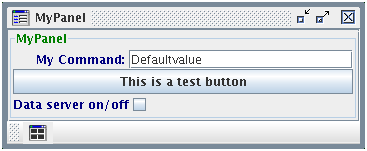
\includegraphics[angle=0,width=.6\textwidth]{prog-minipanel.png} % pdf file
\caption{Minipanel.}
\label{fig:prog-minipanel} % give it a name for references
\end{figure}
That is how the class must look like:
{\small \begin{verbatim}
public class MiniPanel  extends xPanelPrompt
                      implements  xiUserPanel,
                                  ActionListener 
\end{verbatim}
}
The constructor must not have arguments! Icon, name and tooltip have to be
passed by getter function to the caller (the GUI desktop). Layout is mandatory.
Declarations have been masked out in the code snippets.
{\small \begin{verbatim}
public MiniPanel(){
   super("MyPanel");
   menuIcon=xSet.getIcon("Myicon.png");
   name=new String("MyPanel");
   tooltip=new String("Launch my panel");
   layout = xSet.getLayout(name);
   if(layout == null)
   layout=xSet.createLayout(name,new Point(100,200), new Dimension(100,75),1,true);
}
\end{verbatim}
}
The simple functions to be implemented for the interface \class{xiUserPanel}
(we do not provide a command formatting function) are:
{\small \begin{verbatim}
public String getToolTip(){return tooltip;}
public String getHeader(){return name;}
public ImageIcon getIcon(){return menuIcon;}
public xLayout checkLayout(){return layout;}
public xiUserCommand getUserCommand(){return null;}
\end{verbatim}
}
The \func{init} is called once after constructor. Here we have to setup all panels.
We have in the main panel three lines: one text prompt, a text button, and a check box.
At the bottom we have one icon button which would open the display frame.
{\small \begin{verbatim}
public void init(xiDesktop desktop, ActionListener al){
desk=desktop; // save
prompt=addPrompt("My Command: ","Defaultvalue","prompt",20,this);
addTextButton("This is a test button","button","Tool tip, whatever it does",this);
check=addCheckBox("Data server on/off","check",this);
graphIcon   = xSet.getIcon("icons/usergraphics.png");
addButton("Display","Display info",graphIcon,this);
state = new xState("ServerState", xState.XSIZE,xState.YSIZE);
stapan=new xPanelGraphics(new Dimension(160,50),1); // one column of states
metpan=new xPanelGraphics(new Dimension(410,14),1); // one columns of meters
franame=new String("MyGraphics");
fralayout = xSet.getLayout(franame);
if(fralayout == null)
fralayout=xSet.createLayout(franame,new Point(400,400), new Dimension(100,75),1,true);
frame=new xInternalCompound(franame,graphIcon,0,fralayout,xSet.blueD());
}
\end{verbatim}
}
Here we have the callback function for the interactive elements,
the text prompt, the button, the checker, and the icon:
{\small \begin{verbatim}
private void print(String s){
System.out.println(s);
}
public void actionPerformed(ActionEvent e) {
String cmd=e.getActionCommand();
if ("prompt".equals(cmd)) {
  print(cmd+":"+prompt.getText()+" "+check.isSelected());
} else if ("button".equals(cmd)) {
  print(cmd+":"+prompt.getText()+" "+check.isSelected());
} else if ("check".equals(cmd)) {
  print("Data server "+check.isSelected());
  if(check.isSelected()){
    if(param != null)param.setParameter("0");
    state.redraw(0,"Green","Active",true);
  } else {
    if(param != null)param.setParameter("1");
    state.redraw(0,"Gray","Dead",true);
}} else if ("Display".equals(cmd)) {
  if(!desk.findFrame(franame)){
    frame=new xInternalCompound(franame,graphIcon,0,fralayout,xSet.blueD());
    frame.rebuild(stapan, metpan); 
    desk.addFrame(frame); 
}}
}
\end{verbatim}
}
\begin{figure}[htb]
\centering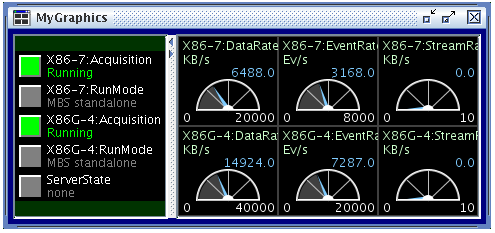
\includegraphics[angle=0,width=.7\textwidth]{prog-ministates.png} % pdf file
\caption{Ministates.}
\label{fig:prog-ministates} % give it a name for references
\end{figure}
With the checker we toggle the \class{xState} state {\keyw{ServerState} in screen shot).
The \class{xiDimParameter} param to be toggled we will find in the next.
To get access to DIM parameters we must implement \func{setDimServices}.
We suggest that there is a parameter \param{*Setup\_File*} which has a string value.
{\small \begin{verbatim}
public void setDimServices(xiDimBrowser browser){
Vector<xiDimParameter> vipar=browser.getParameters();
for(int i=0;i<vipar.size();i++){
  xiParser p=vipar.get(i).getParserInfo();
  String pname=new String(p.getNode()+":"+p.getName());
  if(p.isRate()){ 
      xMeter meter=new xMeter(xMeter.ARC,
        pname,0.0,10.0,xMeter.XSIZE,xMeter.YSIZE,xSet.blueL());
      meter.setLettering(p.getNode(),p.getName(),
        vipar.get(i).getMeter().getUnits(),"");
      metpan.addGraphics(meter,false); 
      browser.addInfoHandler(vipar.get(i),
        new myInfoHandler(pname,meter,null));
  } else if(p.isState()){ 
     xState state=new xState(pname,xState.XSIZE,xState.YSIZE);
     stapan.addGraphics(state,false);
     browser.addInfoHandler(vipar.get(i),
        new myInfoHandler(pname,null,state));
  } else if(p.getFull().indexOf("Setup_File")>0) param=vipar.get(i);
} // end list of parameters
stapan.addGraphics(state,false);
stapan.updateAll();
metpan.updateAll();
if(frame != null) frame.rebuild(stapan, metpan);
\end{verbatim}
}
All references or allocated objects from \func{setDimServices} we have to free in
\func{releaseDimServices}:
{\small \begin{verbatim}
public void releaseDimServices(){
    metpan.cleanup();
    stapan.cleanup();
    param=null;
}
\end{verbatim}
}
We provide a little extra class implementing \class{xiUserHandler} function \func{infoHandler}.
Each parameter we want to monitor gets its own handler instance which has direct
access to our graphics panels.
{\small \begin{verbatim}
private class myInfoHandler implements xiUserInfoHandler{
private myParameter(String Name, xMeter Meter, xState State){
name = new String(Name); // store
meter=Meter; // store
state=State; // store
}
public String getName(){return name;}
public void infoHandler(xiDimParameter P){
if(meter != null) meter.redraw(
   P.getMeter().getValue(),
   true, true);
if(state != null) state.redraw(
   P.getState().getSeverity(),
   P.getState().getColor(),
   P.getState().getValue(),
   true);
}
}
\end{verbatim}
}
\subsection{Store/restore layout}
It is absolutely necessary to save and restore window layouts to be able to see the GUI after
restart as before. This is done through \class{xLayout} objects which are managed centrally.
They keep information about frame position, size, visibility, and the number of columns
in graphics panels. All existing layouts are stored with the save setup button, and restored
on startup.



